\providecommand{\additionalOptionsForClass}{}
\documentclass[
  accentcolor=tud1c,	% Color theme for TUD corporate design
  colorbacktitle,		% Titlepage has colored background for title area
  inverttitle,			% Font color of title on titlepage is inverted
  \additionalOptionsForClass
  %german%,
  %twoside
]{tudexercise}

\parindent1em
%\parskip2ex

\usepackage[ngerman]{babel}
\usepackage[utf8]{inputenc}
\usepackage{listings}
\usepackage{booktabs}
\usepackage{amsmath}
\usepackage{algorithm2e}
\usepackage{hyperref}
\usepackage{xspace}
\usepackage{tabularx}
\usepackage{tikz}
\usepackage{cleveref}
\usepackage{numprint}
\usepackage{paralist}
\usepackage{verbatim}
\usepackage{tocloft} % for manipulating the table of contents

\usetikzlibrary{shapes}
\usetikzlibrary{calc}
\usetikzlibrary{arrows}
\usetikzlibrary{decorations}

\usepackage{pifont}
\newcommand{\cmark}{\ding{51}\xspace}%
\newcommand{\xmark}{\ding{55}\xspace}%

\usepackage{todonotes}
%\usepackage[disable]{todonotes} % Use this line to hide all todos

\definecolor{commentgreen}{RGB}{50,127,50}
\lstloadlanguages{C++,[gnu]make}
\lstset{language=C++}
\lstset{captionpos=b}
\lstset{tabsize=3}
\lstset{breaklines=true}
\lstset{basicstyle=\ttfamily}
\lstset{columns=flexible}
\lstset{keywordstyle=\color{purple}}
\lstset{stringstyle=\color{blue}}
\lstset{commentstyle=\color{commentgreen}}
\lstset{otherkeywords=\#include}
\lstset{showstringspaces=false}
\lstset{keepspaces=true}
\lstset{xleftmargin=1cm}
\lstset{literate=%
	{Ö}{{\"O}}1
	{Ä}{{\"A}}1
	{Ü}{{\"U}}1
	{ß}{{\ss}}2
	{ü}{{\"u}}1
	{ä}{{\"a}}1
	{ö}{{\"o}}1
	{'}{{\textquotesingle}}1
}

\lstnewenvironment{lstmake} %
{\lstset{language=[gnu]make}} %
{}


\newcommand{\superscript}[1]{\ensuremath{^{\textrm{#1}}}}
\newcommand{\subscript}[1]{\ensuremath{_{\textrm{#1}}}}

\newcommand{\setHeader}[1]{
\providecommand{\examheadertitle}{TODO: Titel einbinden}
\renewcommand{\examheadertitle}{#1}
\begin{examheader}
    \examheadertitle
\end{examheader}
}

\newcommand{\hints}[1]{
\paragraph*{Hinweise}
	\begin{itemize}
		\setlength{\itemsep}{0pt}
		#1
	\end{itemize}
}

\newcommand{\optional}{\xspace(optional)}
\newcommand{\experimental}{\xspace(experimentell)}

\usepackage{fancybox}
\newcommand{\optionaltextbox}{
	\bigskip
	\begin{center}
		\ovalbox{\parbox{0.98\textwidth}{Die Klausur kann ohne diese Aufgabe bestanden werden. Wir empfehlen aber sie trotzdem zu bearbeiten.}}
	\end{center}
}
\newcommand{\experimentaltextbox}{
	\bigskip
	\begin{center}
		\ovalbox{\parbox{0.98\textwidth}{Diese Aufgabe wurde neu erstellt und kann noch Fehler und Inkonsistenzen enthalten. Falls euch etwas derartiges auffällt sprecht uns bitte darauf an oder stellt es auf GitHub in den Issuetracker unter \url{https://github.com/Echtzeitsysteme/tud-cpp-exercises/issues}}}
	\end{center}
}

\newcommand{\enquote}[1]{\glqq#1\grqq\xspace}
\newcommand{\filename}[1]{\texttt{#1}}

\newcommand{\RK}[1]{\todo[]{\textbf{RK:} #1}}
\newcommand{\RKi}[1]{\todo[inline]{\textbf{RK:} #1}}

\newcommand{\ExercisePrefix}[1]{$[$#1$]$ \xspace}
\newcommand{\ExercisePrefixBasics}{\ExercisePrefix{G}}
\newcommand{\ExercisePrefixMemory}{\ExercisePrefix{S}}
\newcommand{\ExercisePrefixObjectOrientation}{\ExercisePrefix{O}}
\newcommand{\ExercisePrefixAdvanced}{\ExercisePrefix{F}}
\newcommand{\ExercisePrefixEmbeddedC}{\ExercisePrefix{C}}
\newcommand{\ExercisePrefixElevator}{\ExercisePrefix{A}}
\newcommand{\ExercisePrefixAdditionalInformation}{\ExercisePrefix{Z}}


\newcommand{\exday}{2}

\cppSetTitle

\begin{document}

\cppSetHeaderAndMakeTitle



\section{Zeiger und Referenzen Grundlagen}

\subsection{Experimente}
Experimentiere mit Zeigern, Adressen und Referenzen.
Mache dir eine Skizze, die verdeutlicht, wie Variablen und ihre Speicherabbilder zusammenhängen.
Als Ausgangsbasis kann folgendes Programmfragment dienen.

\begin{lstlisting}
int intVal = 42;
int *pIntVal = &intVal;
cout << "Wert von IntVal " << intVal << endl;
cout << "Wert von &IntVal " << &intVal << endl;
cout << "Wert von pIntVal " << pIntVal << endl;
cout << "Wert von *pIntVal " << *pIntVal << endl;
cout << "Wert von &pIntVal " << &pIntVal << endl;
\end{lstlisting}

\subsection{Bedeutung verstehen}
Seien \texttt{intVal} und \texttt{pIntVal} wie oben gegeben.
Versuche die Bedeutung folgender Ausdrücke zu verstehen.
Welche Regelmäßigkeiten stellst du fest?

\begin{lstlisting}
*&intVal;
*&pIntVal;
&*pIntVal;
**&pIntVal;
*&*&intVal;
&*&pIntVal;
*&*pIntVal;
\end{lstlisting}

\hints{
	\item Gehe dabei von innen nach außen vor.
}


\subsection{Gültigkeit}
Warum sind folgende Ausdrücke ungültig?

\begin{lstlisting}
*intVal;
**pIntVal;
**&*pIntVal;
&*intVal;
&42;
\end{lstlisting}

\hints{
	\item Finde heraus, welchen Typ der Ausdruck hätte haben müssen.
	\item Nur tatsächlich angelegte Variablen haben Adressen. Ausdrücke wie a + b oder direkt kodierte Zahlenliterale wie 42 haben keine Adresse-
}

\subsection{Variablentausch}
Schreibe eine Funktion \texttt{swap}, die zwei \texttt{int}-Variablen miteinander vertauscht.
Probiere dabei beide möglichen Übergabevarianten (per Referenz, per Pointer) aus.

\subsection{Programmanalyse}
Sieh dir folgendes Programm an.

\vbox{%fixes empty page
\begin{lstlisting}
#include <iostream>

void foo(int &i) {
	int i2 = i;
	int &i3 = i;
	
	std::cout << "i = " << i << std::endl;
	std::cout << "i2 = " << i2 << std::endl;
	std::cout << "i3 = " << i3 << std::endl;
	std::cout << "&i = " << &i << std::endl;
	std::cout << "&i2 = " << &i2 << std::endl;
	std::cout << "&i3 = " << &i3 << std::endl;
}

int main() {
	int var = 42;
	std::cout << "&var = " << &var << std::endl;
	foo(var);
}
\end{lstlisting}
}

Welche Adressen werden übereinstimmen, welche werden sich unterscheiden?
Führe das Programm aus.
Hast du diese Ausgabe erwartet?



\newpage

\section{Arrays und Zeigerarithmetik}
Arrays sind zusammenhängende Speicherbereiche, die mehrere Variablen von gleichem Typ speichern können.
Arrays werden in C++ folgendermaßen angelegt: \texttt{<Typ> <name>[<Größe>];}, zum Beispiel:

\begin{lstlisting}
	int arr[10];	// array of 10 integers
\end{lstlisting}

Falls das Array global ist, muss die Größe eine konstante Zahl sein, falls das Array in einer Funktion auf dem Stack angelegt wurde, kann die Größe auch durch eine Variable vorgegeben werden.
Auf jeden Fall bleibt diese während der Existenz des Arrays konstant und kann sich nach dem Anlegen nicht mehr ändern.

Ein Array kann direkt bei der Deklaration initialisiert werden:

\begin{lstlisting}
	int arr[5] = {1, 2, 3, 4, 5};
\end{lstlisting}

Man kann die Größe optional auch weglassen, in diesem Fall wird sie der Compiler anhand der angegebenen Elemente selbst ermitteln.

Man kann auf die einzelnen Elemente des Arrays wie gewohnt über \textbf{arr[i]} zugreifen.

Arrays und Zeiger sind in C++ stark miteinander verwandt.
So ist der \textbf{Bezeichner} des Arrays gleichzeitig die \textbf{Adresse des ersten Elements}.
Somit kann man sowohl durch \textbf{*arr} als auch durch \textbf{arr[0]} auf das erste Element zugreifen.
Analog dazu kann man auch einen Zeiger auf das erste Element anlegen:

\begin{lstlisting}
	int *pArr = arr;
\end{lstlisting}

Da die Elemente eines Array direkt hintereinander stehen, kann man den Zeiger inkrementieren, um zum  nächsten Element zu gelangen.
Beispiel:

\begin{lstlisting}
	int *pArr = arr;
	std::cout << "Address of first element: "  << pArr << std::endl;
	std::cout << "Address of second element: " << pArr+1 << std::endl;
	std::cout << "Address of third element: "  << pArr+2 << std::endl;
\end{lstlisting}

Somit kann man auf beliebige Elemente des Array über den Zeiger zugreifen:

\begin{lstlisting}
	*(pArr + 0);	// first element
	*(pArr + 1);	// second element
	*(pArr + 2);	// third element
	*(pArr + i);	// ith element
	++pArr;			// increment pointer by 1
	*(pArr + 0);	// second(!!) element of arr
	*(pArr + 2);	// fourth(!!) element of arr
\end{lstlisting}

Tatsächlich ist \textbf{*(p+i)} in \textbf{jeder Hinsicht äquivalent} zu \textbf{p[i]}.
Das bedeutet, dass man sowohl auf das i-te Element eines Arrays über \textbf{*(arr + i)} zugreifen kann als auch über \textbf{pointer[i]} auf das Element, auf welches der Zeiger \texttt{pointer+i} zeigt!

In C++ findet keine automatische Bereichsprüfung bei Arrayzugriffen statt.
Du bist als Programmierer selbst dafür verantwortlich, dass niemals auf ein Element außerhalb der Array-Grenze zugegriffen wird.
Falls doch, kann es zu Programmabstürzen oder unerwünschten Effekten wie  Buffer-Overflows kommen, die ein erhebliches Sicherheitsrisiko darstellen.
Bevorzuge deshalb Container-Klassen wie \texttt{std::vector} (oder \texttt{std::array} ab C++11) aus der Standardbibliothek anstelle von \glqq rohen\grqq{} Arrays.
Beachte außerdem, dass der Operator \textbf{delete[]} zwar das Array löscht, den Zeiger jedoch \textbf{nicht} auf \emph{NULL} setzt.
Dabei entsteht ein \emph{Dangling Pointer}, welcher dazu führen kann, dass später im Programm auf Speicherstellen zugegriffen wird, die nicht reserviert sind.
Setze deshalb Zeiger nach einem \textbf{delete/delete[]} sofort auf \texttt{NULL}, um Speicherfehler zu vermeiden.

Um die Größe eines Arrays zu ermitteln, kannst du den \texttt{sizeof()}-Operator benutzen. Dieser gibt generell die Anzahl der Bytes an, die eine Variable verbraucht. Da einzelne Array-Elemente größer als ein Byte sein können, muss die Gesamtgröße des Arrays durch die Größe eines Elements geteilt werden, um auf die Anzahl der Elemente zu kommen.

\begin{lstlisting}
	int arr[10];
	std::cout << sizeof(arr) << std::endl; // 40 on 32-bit machine, 80 on 64-bit
	int len = sizeof(arr) / sizeof(arr[0]);
	std::cout << len << std::endl; // always 10
\end{lstlisting}

Beachte, dass \texttt{sizeof()} \textbf{nicht} dazu verwendet werden kann, um die Größe des Arrays herauszufinden, auf die ein Zeiger zeigt.
In diesem Fall wird \texttt{sizeof()} nämlich die \textbf{Größe des Zeigers} und nicht die Größe des Arrays liefern!

\begin{lstlisting}
	int arr[10];
	int *pArr = arr;
	std::cout << sizeof(pArr) << std::endl; // 4 on 32-bit machine, 8 on 64-bit
\end{lstlisting}

\subsection{}
Lege in der \texttt{main}-Funktion ein \texttt{int}-Array mit 10 Elementen an, und initialisiere es mit den Zahlen 1 bis 10.
Iteriere in einer Schleife über das Array und gib alle Elemente nacheinander aus.

\subsection{}
In C und C++ kann man Arrays nicht direkt an Funktionen übergeben.
Stattdessen übergibt man einen Zeiger auf das erste Element des Arrays. Aufgrund der Äquivalenz von \textbf{*(p+i) } und \textbf{p[i]} kann man in der Funktion den Zeiger syntaktisch wie das Original-Array verwenden.

Schreibe eine Funktion, die einen \texttt{const}-Zeiger auf das erste Element eines Arrays bekommt und alle Elemente ausgibt.
Da die Funktion nur anhand des Zeigers keine Möglichkeit hat zu wissen, wie groß das Array ist, muss die Größe des Arrays durch einen weiteren Parameter übergeben werden\footnote{Statt \texttt{unsigned int} wird oft der Standard-Typ \texttt{size\_t} genutzt (z.B. in \texttt{std::vector}).}:

\begin{lstlisting}
	void printElements(const int *const array, const unsigned int size);
\end{lstlisting}

\subsection{}
Wie wir vorher gesehen haben, kann man mit Zeigern auch rechnen und diese nachträglich ändern.
Anstatt mit einem Index das Array zu durchlaufen, kann man stattdessen bei jeder Iteration den Zeiger selbst inkrementieren!

\begin{lstlisting}
	for(const int *p = array; p != array + 10; ++p) {
		// *p contains current element
		// ...
	}
\end{lstlisting}

Schreibe die Funktion aus der vorherigen Aufgabe so um, dass sie einen laufenden Zeiger anstatt eines Indexes verwendet.

\subsection{}
Ebenso kann man auch die Arraygröße auf eine andere Weise übergeben, indem man die Adresse des Elements nach dem letzten Element angibt.
Dadurch werden Schleifen der Form

\begin{lstlisting}
	for(const int *p = begin; p != end; ++p) {
		// *p contains current element
		// ...
	}
\end{lstlisting}

möglich.
Schreibe die Funktion aus der vorherigen Aufgabe entsprechend um.
Vergiss nicht, den Zeiger als \texttt{const} zu definieren, da Elemente nur gelesen werden.
Du kannst hier \texttt{const} doppelt verwenden, um auch sicherzustellen, dass der \texttt{end}-Zeiger nicht verändert wird.

\subsection{}
Die obige Methode, über Elemente eines Arrays zu iterieren, mag dir zunächst etwas ungewöhnlich erscheinen.
Sie hat jedoch den Vorteil, dass man anstatt des ganzen Arrays auch kleinere zusammenhängende Teile davon an Funktionen übergeben kann, indem man Zeiger auf die entsprechenden Anfangs-und Endelemente setzt.
Beispiel:

\begin{lstlisting}
	int arr[10];
	printElements(arr+5, arr+8); // Print elements with index 5, 6, 7
\end{lstlisting}

Experimentiere etwas mit dieser Übergabemethode in deiner eigenen Funktion!

\subsection{}
Bisher haben wir das Array auf dem Stack angelegt
Mit \textbf{new[]} kann man ein Array auf dem Heap erzeugen.
Dabei wird die Adresse des ersten Elements in einem Zeiger gespeichert.
Mittels \textbf{delete[]} \textbf{muss} man den belegten Speicher nach Benutzung freigeben.
Beispiel:

\begin{lstlisting}
	int *pArr = new int[10]; // size can be a variable
	doSomethingWith(pArr, 10);
	delete[] pArr; // <-- notice the [] !
\end{lstlisting}

Beachte die \textbf{[]} nach delete.
Diese bewirken, dass das gesamte Array und nicht bloß das erste Element gelöscht wird.

Ein Anwendungsfall von dynamischen Arrays sind Funktionen, die ein Array von vorher unbekannter Größe zurückgeben.
Schreibe eine Funktion, die beliebig viele Zahlen von der Konsole mittels \texttt{std::cin} einliest.
Der Benutzer soll dabei zuvor gefragt werden, wie viele Zahlen er eingeben möchte.
Speichere die Zahlen in einem dynamisch angelegten Array ab und lasse die Funktion einen Zeiger darauf zurückgeben.
Hier ist ein Beispiel wie \texttt{std::cin} zu verwenden ist:

\begin{lstlisting}
unsigned int size;
std::cout << "Größe: ";
std::cin >> size;
std::cout << "Gewählte Größe: " << size << std::endl;
\end{lstlisting}

Zusätzlich zum Zeiger muss die Funktion auch die Möglichkeit haben, ihrem Aufrufer die Größe des angelegten Arrays mitzuteilen.
Füge der Funktion deshalb einen weiteren Parameter hinzu, in dem entweder per Referenz oder per Zeiger eine Variable übergeben wird, um dort die Größe abzulegen\footnote{Du merkst sicherlich schon jetzt, dass es umständlich/fehleranfällig ist, wenn man die Größe eines Arrays separat speichern und übergeben muss.}.

Gib die eingelesenen Werte auf der Konsole aus.
Vergiss nicht, am Ende den Speicher freizugeben.



\newpage

\section{Verkettete Listen}
In dieser Aufgabe wollen wir eine doppelt verkettete Liste von Integern implementieren.
Dazu brauchen wir zwei Klassen:
\texttt{ListItem} stellt ein Element der Liste mit dessen Inhalt dar und \texttt{List} speichert die Zeiger auf Anfangs- und Endelemente und bildet den eigentlichen Zugangspunkt für die Liste.

\begin{center}
	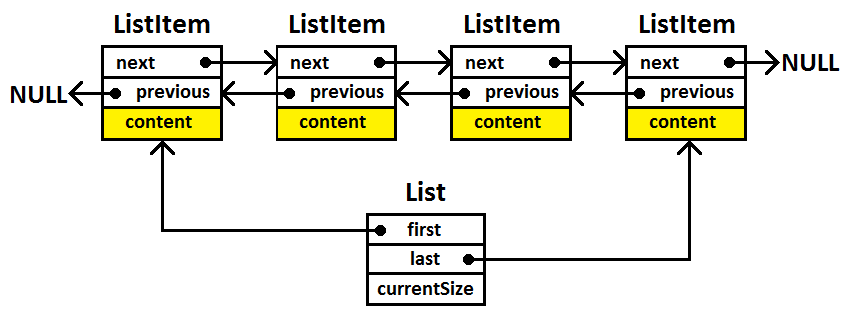
\includegraphics[width=.7\textwidth]{figures/list.png}
\end{center}

Wir werden am Tag 4 auf dieser Aufgabe aufbauen und die Liste um weitere Funktionen erweitern.
Behalte dies bitte im Hinterkopf und lösche deine Lösung nicht.
Falls du mit dieser Aufgabe bis dahin nicht fertig sein solltest, kannst du natürlich auch die Musterlösung als Ausgangspunkt nehmen.

\subsection{Klasse \texttt{ListItem}}
Implementiere die Klasse \texttt{ListItem}, welche die zu speichernde Zahl sowie Verweise auf das vorherige und nächste \texttt{ListItem} als Attribute hat.
Verwende dazu Zeiger und keine Referenzen, da Referenzen nachträglich nicht mehr geändert werden können.
Auch können Referenzen nicht \emph{NULL} sein, was in unserem Fall nötig ist, um zu markieren, dass ein Element keine Vorgänger oder Nachfolger hat.

Der Konstruktor sollte sowohl seine eigenen \texttt{next} und \texttt{previous} Zeiger initialisieren, als auch die seiner Vorgänger- und Nachfolgerelemente.
Die Methode \texttt{getContent()} soll eine Referenz auf den Inhalt zurückgeben, damit dieser durch eine Zuweisung modifiziert werden kann.

\begin{lstlisting}
class ListItem {
public:
	/**
	 * create a list item between two elements with a given given content
	 * (also modify previous->next and next->previous)
	 */
	ListItem(ListItem *prev, ListItem *next, int content);
	/**
	 * delete this list item (also change previous->next and next->previous
	 * to not point to this item anymore)
	 */
	~ListItem();				
	int& getContent();			// get a reference to the contained data
	ListItem* getNext();			// get the next list item or NULL
	ListItem* getPrevious();	// get the previous list item or NULL
private:
	ListItem *previous;		// previous item in list
	ListItem *next;			// next item in list
	int content;				// content of this list item
};
\end{lstlisting}

\subsection{Privater Copy-Konstruktor}
Unsere \texttt{ListItem} Klasse hat einen kleinen Design-Fehler:
Da wir keinen Copy-Konstruktor definiert haben, generiert der Compiler automatisch einen.
Dieser kopiert einfach die einzelnen Attribute des Ursprungsobjekts (Shallow Copy).
In unserem Fall ergibt das Kopieren eines Items jedoch semantisch keinen Sinn, weil dabei ein hängendes \texttt{ListItem} entstehen würde, welches nicht mit der Liste verknüpft ist, aber dennoch auf andere Items der Liste zeigt.

Deshalb werden wir das Kopieren von \texttt{ListItem}-Objekten verbieten, indem wir einen privaten Copy-Konstruktor deklarieren, ohne ihn zu implementieren.
Dadurch kann der Copy-Konstruktor nie aufgerufen werden und der Compiler kann dies zur Compilezeit überprüfen.

Implementiere einen leeren privaten Copy-Konstruktor.

\begin{lstlisting}
private:
	/** Private copy constructor (without implementation)*/
	ListItem(const ListItem& other);
\end{lstlisting}

\subsection{Klasse \texttt{List}}
Implementiere nun die Klasse \texttt{List}.
Achte bei den Methoden zum Einfügen und Entfernen von Elementen darauf, dass bei einer leeren Liste eventuell sowohl die \texttt{first} als auch \texttt{last} Zeiger modifiziert werden müssen.
Vergiss nicht, \texttt{currentSize} bei jeder Operation entsprechend anzupassen.
Falls die Liste leer ist, sollten \texttt{deleteFirst()} und \texttt{deleteLast()} einfach nichts ändern\footnote{Lieber würde man hier einen Fehler werfen, aber Exceptions haben wir an dieser Stelle noch nicht behandelt.}.

\begin{lstlisting}
class List {
public:
	List();								// create an empty list
	~List();								// delete the list and all of its elements
	List(const List& other);		// create a copy of another list
	void appendElement(int i);		// append an element to the end of the list
	void prependElement(int i);	// prepend an element to the beginning of the list
	void insertElementAt(int i, int pos);	// insert an element i at position pos
	int getSize() const;				// get the number of elements in list
	int& getNthElement(int n);		// get the n-th element.
	int& getFirst();					// get the first element
	int& getLast();					// get the last element
	int deleteFirst();			// delete first element and return it (return 0 if empty)
	int deleteLast();				// delete last element and return it (return 0 if empty)
	int deleteAt(int pos);		// delete element at position pos
private:
	ListItem *first, *last;		// first and last item pointers (NULL if list is empty)
	int currentSize;				// current size of the list
};
\end{lstlisting}

\subsection{}
Teste deine Implementation.
Füge der Liste Elemente von beiden Seiten hinzu und lösche auch wieder welche.
Kopiere die Liste und gib die Elemente nacheinander aus.

\subsection{}
Bisher haben wir über \texttt{getNthElement()} auf die Elemente der Liste zugegriffen.
Diese Methode kann insbesondere bei langen Listen sehr langsam sein.
Deshalb werden wir einen Iterator schreiben, über den man auf die Listenelemente sequentiell zugreifen kann.
Der Iterator soll dabei einen Zeiger auf das aktuell betrachtete Element der Liste halten.

Um den Zugriff möglichst komfortabel zu gestalten, werden wir den Iterator als eine Art Zeiger implementieren, den man über \textbf{$++$} und \textbf{$--$} in der Liste verschieben kann.
Um auf ein Element zuzugreifen, überladen wir den Dereferenzierungsoperator $*$.
Somit können wir unsere Liste ähnlich zu \texttt{std::vector} verwenden:
\begin{lstlisting}
	for (ListIterator iter = list.begin(); iter != list.end(); iter++) {
		cout << *iter << endl;
	}
\end{lstlisting}

Beginne mit einer Grundversion des Iterators.
Erstelle einen Konstruktor, der die Attribute des Iterators (Zeiger auf aktuelles Element und Zeiger auf die Liste) entsprechend initialisiert.
Implementiere den Vergleichsoperator \textbf{!=} sowie den Dereferenzierungsoperator \textbf{*}.
Der Dereferenzierungsoperator solle den Inhalt des aktuellen Items zurückgeben.
Du brauchst nicht zu prüfen, ob \texttt{item} tatsächlich auf ein gültiges Element zeigt (Das machen/können Standardbibliotheksiteratoren übrigens auch nicht!).
Zum Vergleichen zweier Iteratoren prüfen Sie, ob die \texttt{item} und \texttt{list} Zeiger identisch sind.
Vergleiche nicht den Inhalt der Items, da der Vergleich auch dann funktionieren soll, wenn \texttt{item} NULL ist, der Iterator also auf kein Element zeigt.

\begin{lstlisting}
class ListIterator {
public:
	// create a new list iterator pointing to an item in a list
	ListIterator(List* list, ListItem* item);
	// get the content of the current element
	int& operator*();
	// check whether this iterator is not equal to another one
	bool operator!=(const ListIterator& other) const;
private:
	List *list;
	ListItem *item;
};
\end{lstlisting}


Implementiere nun den \textbf{$++$} Operator zum Inkrementieren des Iterators.
Falls der Iterator zuvor auf kein Item zeigte (\texttt{item == NULL}), soll er nun auf das erste Element der Liste gesetzt werden.
Die Prototypen dazu lauten:
\begin{lstlisting}
// Increment this iterator and return itself (prefix ++)
ListIterator& operator++();
// Increment this iterator but return the previous iterator (copy) (postfix ++)
ListIterator operator++(int);
\end{lstlisting}

Bei der Überladung des \textbf{$++$} Operators muss eine Sonderregel beachtet werden.
Dieser Operator kann sowohl als Postfix (z.B. iter$++$) als auch Präfix (z.B. $++$iter) verwendet werden.
Um den Compiler darüber zu informieren, welche Variante wir überladen, wird beim Postfix-Operator ein Dummy-Parameter vom Typ \texttt{int} definiert.
Dieser dient nur der syntaktischen Unterscheidung und hat keine weitere Bedeutung.
Beachte außerdem, dass bei Präfix-Operationen der Iterator sich selbst zurückgeben sollte, während der Postfix-Operationen eine Kopie des Iterators zurückgibt, die auf das vorherige Element zeigt.

Zum besseren Verständnis ist ein Teil der Implementation gegeben:

\begin{lstlisting}
// Prefix ++  ->  increment iterator and return it
ListIterator& ListIterator::operator++() {
	if (item == NULL) {
		item = ...	 // set item to first item of list
	}
	else {
		item = ...	 // set item to next item of current item
	}
	return *this;	 // return itself
}

// Postfix ++  -> return iterator to current item and increment this iterator
ListIterator ListIterator::operator++(int) {
	ListIterator iter(list, item); // Store current iterator
	if (item == NULL) {
		item = ...	 // set item to first item of list
	}
	else {
		item = ...	 // set item to next item of current item
	}
	return iter; 	// return iterator to previous item
}
\end{lstlisting}

Du wirst in den Methoden auf private Attribute der Liste zugreifen müssen. Um dies zu ermöglichen, könnte man öffentliche Getter für die Items der Liste schreiben.
Dadurch würde jedoch jeder die Möglichkeit bekommen, direkt auf die Items der Liste zuzugreifen, was dem Geheimnisprinzip zuwiderläuft.
Deshalb werden wir \texttt{ListIterator} stattdessen explizit erlauben, auf \texttt{private}-Attribute der Liste zuzugreifen.
Dazu müssen wir \texttt{ListIterator} als \texttt{friend} von \texttt{List} deklarieren.
Füge dazu folgende Zeile (an beliebiger Stelle, üblich ist der Anfang der Klasse) zur Klassendefinition von \texttt{List} hinzu:
\begin{lstlisting}
friend class ListIterator;
\end{lstlisting}

Überlade auf die gleiche Weise auch den \textbf{$--$} Operator sowohl in Postfix als auch Präfix-Form.

Nun ist unsere Implementation fast komplett und wir brauchen nur noch Methoden, um Iteratoren zu erzeugen.
Implementiere dazu die folgenden Methoden innerhalb der \texttt{List} Klasse, um Iteratoren auf das erste und letzte Element der Liste zu erzeugen.
\begin{lstlisting}
// return an iterator pointing to the first element
ListIterator begin();
// return an iterator pointing to the element after the last one
ListIterator end();
\end{lstlisting}

Höchstwahrscheinlich wirst du Probleme bei der Kompilierung haben.
Dies liegt an der zirkulären Abhängigkeit zwischen \texttt{List} und \texttt{ListIterator}.
Gehe dazu folgendermaßen vor:
Verschieben die \texttt{\#include} Anweisungen für die Header von \texttt{List} und \texttt{ListItem} aus \texttt{ListIterator.h} nach \texttt{ListIterator.cpp} und füge in \texttt{ListIterator.h} folgendes hinzu

\begin{lstlisting}
class ListItem;
class List;
\end{lstlisting}

Dies sind Vorwärtsdeklarationen (\textbf{Forward Declaration}), die dem Compiler sagen, dass die Klassen existieren, aber später definiert werden. Nun kannst problemlos \texttt{ListIterator.h} in \texttt{List.h} einbinden.

\subsection{}
Teste deine Implementation.
Erstelle eine Liste, füge Elemente hinzu und iteriere über Listenelemente:

\begin{lstlisting}
for (ListIterator iter = list.begin(); iter != list.end(); iter++) {
	cout << *iter << endl;
}
\end{lstlisting}

Warum kann man \textbf{nicht} rückwärts durch die Liste iterieren, indem man einfach die Aufrufe \texttt{list.begin()} und \texttt{list.end()} tauscht und \texttt{iter$--$} statt \texttt{iter$++$} verwendet?
Denke daran, worauf die von \texttt{begin())} und \texttt{end()} zurückgegebenen Iteratoren zeigen.




\newpage

\section{Smart Pointers}
In dieser Aufgabe werden wir uns mit der Benutzung von Smart Pointers vertraut machen. Dazu werden wir die Smart Pointer Klassen \texttt{boost::shared\_ptr} und \texttt{boost::weak\_ptr} der Boost-Bibliothek verwenden.

\subsection{}
Erstellen eine Klasse \texttt{TreeNode}, die einen Knoten eines Binärbaums darstellt.
Jeder Knoten hat einen Inhalt vom Typ \texttt{int} sowie einen Zeiger auf seine beiden Kindknoten.
Statt \glqq roher\grqq{} Zeiger verwenden wir Smart Pointers, die das Speichermanagement übernehmen.
Dadurch wird es nicht nötig sein, Kindknoten manuell zu löschen.
Sie werden automatisch entfernt, sobald der Wurzelknoten gelöscht ist und keine Zeiger mehr auf den Kindknoten zeigen.

\begin{lstlisting}
#include <boost/shared_ptr.hpp>
class TreeNode;

typedef boost::shared_ptr<TreeNode> TreeNodePtr;	// typedef for better reading

class TreeNode {
public:
	/** create a new tree node and makes it shared */
	static TreeNodePtr createNode(int content, TreeNodePtr left = TreeNodePtr(), TreeNodePtr right = TreeNodePtr());
	~TreeNode();
private:
	TreeNode(int content, TreeNodePtr left, TreeNodePtr right);	// create a tree node
	TreeNodePtr leftChild, rightChild;									// left and right child
	int content;																// node content
};
\end{lstlisting}

Der Konstruktor von \texttt{TreeNode} privat, weil nur die Smart Pointer die Verantwortung für die Lebenszeit eines Objektes übernehmen sollen und bestimmen, wann es gelöscht wird.
Würde man \texttt{TreeNode}-Objekte direkt auf dem Stack anlegen, kann es passieren, dass der Objektdestruktor mehrmals aufgerufen wird -- einmal vom Smart Pointer und einmal beim Verlassen der Funktion.
Ebenso sollten wir keine Rohzeiger auf das Objekt erzeugen, da diese das Speichermanagement der Smart Pointer umgehen.
Stattdessen stellen wir eine statische Methode bereit, um \texttt{TreeNode}-Objekte auf dem Heap zu erzeugen und diese direkt einem Smart Pointer zu übergeben.

Implementiere den Konstruktor, Destruktor sowie \texttt{createNode}.
Der Konstruktor sollte die Attribute entsprechend initialisieren.
Schreibe auch eine Textausgabe, die den Zeitpunkt der Erzeugung eines \texttt{TreeNode}s deutlich macht.
Der Destruktor braucht die Kindknoten nicht zu löschen, da dies bei der Zerstörung des Elternknotens automatisch geschieht.
Füge auch hier eine Textausgabe ein, die die Zerstörung des Objekts sichtbar macht.

Das Schlüsselwort \textbf{static} sowie die Default-Parameter müssen bei der Implementation der Methode ausgelassen werden.
Der Smart Pointer für die Rückgabe wird mit einem Zeiger auf ein \texttt{TreeNode}-Objekt initialisiert. Somit lautet der Methodenrumpf

\begin{lstlisting}
TreeNodePtr TreeNode::createNode(int content, TreeNodePtr left, TreeNodePtr right) {
	return TreeNodePtr(new TreeNode(...));
}
\end{lstlisting}

\subsection{}
Teste, ob die einzelnen Knoten tatsächlich gelöscht werden, sobald kein Zeiger mehr auf den Elternknoten zeigt.
Erstelle dafür einen kleinen Baum:

\begin{lstlisting}
TreeNodePtr node = TreeNode::createNode(1, TreeNode::createNode(2), TreeNode::createNode(3));
\end{lstlisting}

Führe das Programm aus und beobachte die Ausgabe.
Sobald \texttt{main} verlassen wird, wird der Zeiger \texttt{node} gelöscht, und somit auch das dahinterliegende \texttt{TreeNode}-Objekt mit all seinen Kindknoten.

Um ganz sicher zu gehen, dass der Baum tatsächlich beim Löschen des letzten Zeigers zerstört wurde und nicht etwa durch das Beenden des Programms, kannst du \texttt{node} mit einem anderen Baum überschreiben.
Füge in diesem Fall am Ende des Programms eine Textausgabe hinzu, damit ersichtlich wird, dass der erste Baum noch vor Verlassen der \texttt{main} gelöscht wurde.

\subsection{}
Nun wollen wir \texttt{TreeNode} so erweitern, dass jeder Knoten Kenntnisse über seinen Elternknoten besitzt.
Füge das Attribut

\begin{lstlisting}
	TreeNodePtr parent;		// parent node
\end{lstlisting}

hinzu.
Da der Elternknoten beim Erzeugen eines \texttt{TreeNode}s undefiniert ist, brauchst du den Konstruktor nicht zu ändern. \texttt{parent} wird dann automatisch mit NULL initialisiert.

Implementiere die folgende Methode, die einem Knoten seinen Elternknoten zuweist:

\begin{lstlisting}
	void setParent(const TreeNodePtr &p);		// set parent of this node
\end{lstlisting}

\emph{Hinweis}:
\texttt{p} wird in diesem Fall nur deshalb als \texttt{const} Referenz übergeben, da es verhältnismäßig aufwändig ist, einen Smart Pointer zu kopieren.
Beachte, dass im obigen Fall der Smart Pointer selbst const ist, und nicht das Objekt, worauf er zeigt.

Jetzt muss noch \texttt{createNode()} modifiziert werden, sodass \texttt{setParent()} auf den Kindknoten aufgerufen wird. Da ein Smart Pointer die Operatoren $*$ und $->$ überladen hat, lässt er sich syntaktisch wie ein normaler Zeiger benutzen. Um zu überprüfen, ob ein Smart Pointer auf ein Objekt zeigt, kann dieser implizit nach \texttt{bool} gecastet werden. Somit lautet die neue Implementation von \texttt{createNode()}:

\begin{lstlisting}
TreeNodePtr TreeNode::createNode(int content, TreeNodePtr left, TreeNodePtr right) {
	TreeNodePtr node(new TreeNode(content, left, right));
	if (left) {
		left-> ... ; // set parent node
	}
	if (right) {
		right-> ... ; // set parent node
	}
	return node;
}
\end{lstlisting}

\subsection{}
Teste deine Implementation.
Du brauchst dazu in \texttt{main} nichts zu ändern.

Erschreckenderweise siehst du nun, dass überhaupt keine \texttt{TreeNode}-Objekte mehr gelöscht werden.
Die Ursache dafür ist die zirkuläre Abhängigkeit zwischen Kind- und Elternknoten.
Denn selbst wenn sie keine Zeiger auf den Wurzelknoten eines Baumes haben, verweisen die Kindknoten noch immer darauf.

Um dieses Problem zu lösen, müssen die Verweise zum Elternknoten \emph{schwach} (weak) sein.
Ein Knoten darf gelöscht werden, wenn nur noch schwache Zeiger (oder keine) auf ihn verweisen.
Binde dazu den Header \texttt{boost/weak\_ptr.hpp} ein und erstelle ein neues \texttt{typedef} für einen schwachen \texttt{TreeNode} Smart Pointer:

\begin{lstlisting}
typedef boost::weak_ptr<TreeNode> TreeNodeWeakPtr;
\end{lstlisting}

Ändere nun den Typ von \texttt{parent} auf \texttt{TreeNodeWeakPtr}.
Es müssen keine weiteren Änderungen gemacht werden, da starke Zeiger (\texttt{shared\_ptr}) implizit in schwache Zeiger (\texttt{weak\_ptr}) umgewandelt werden können.

\subsection{}
Teste deine Implementation.
Nun sollte sich \texttt{TreeNode} wie gewünscht verhalten.



\newpage

\section{Fortsetzung Aufzug}
In dieser Aufgabe erweitern und verbessern wir unseren Aufzugsimulator, sodass das Kopieren von Personen wegfällt.
Dies werden wir erreichen, indem wir nicht direkt mit \texttt{Person}-Objekten oder -rohzeigern sondern mit Smart Pointern arbeiten.
Dadurch müssen wir beim Verschieben von Personen in den Aufzug nur die Smart Pointer kopieren, während die \texttt{Person}-Objekte selbst bestehen bleiben.

Ein weiterer Vorteil ist, dass wir von jeder Person genau ein Exemplar im Speicher halten.
Möchten wir beispielsweise den Namen einer Person ändern, ist dies überall, wo die Person auftaucht sofort und konsistent sichtbar.
Nutzt man überall Kopien von Personen, haben wir keine Kontrolle darüber und wären gezwungen die Klasse \texttt{Person} immutabel zu machen.

\hints{
	\item In der nächsten Aufgabe hast du die Möglichkeit, die Performanz der alten und der neuen Implementation zu vergleichen.
	Dazu ist es nötig, dass du jetzt eine Kopie von deinem aktuellen Code machst.
	In Eclipse kannst du ganze Projekte per Copy \& Paste kopieren.
}

\subsection{Refactoring mit Referenzen und \texttt{const}}
Als Erstes verbessern wir die Sauberkeit des vorhandenen Codes mithilfe der bisher kennengelernten Mittel wie Referenzen und \texttt{const}.
Es ist sinnvoll, dass du die Änderungen stückweise im Code durchführst und zwischendurch testest, ob alles noch korrekt funktioniert.

Deklariere dafür sämtliche Getter in \texttt{Building}, \texttt{Elevator}, \texttt{Floor} und \texttt{Person} als \texttt{const}, z.B. \texttt{Building::getFloor()} und \texttt{Elevator::getEnergyConsumed()}.
Passe außerdem die Methode \texttt{Elevator::addPeople()} so an, dass die Liste \texttt{people} nicht mehr als Wert sondern als \texttt{const} Referenz übergeben wird.

\hints{
	\item Um über eine \texttt{const} Liste zu iterieren, verwende \texttt{vector<T>::const\_iterator} anstatt \texttt{vector<T>::iterator} als Iterator-Typ.
}

\subsection{}
Binde in deinem Projekt den Boost-Ordner in den Include-Pfad des Compilers ein (siehe vorige Aufgabe).

\subsection{}
Um nicht immer wieder \texttt{boost::shared\_ptr<Person>} schreiben zu müssen, definiere ein \texttt{typedef PersonPtr} für diesen Typen.
Binde den Header \texttt{boost/shared\_ptr.hpp} in \texttt{Person.h} ein und definiere den neuen Typen \texttt{PersonPtr} hinter der Klassendefinition von \texttt{Person}:

\begin{lstlisting}
typedef boost::shared_ptr<Person> PersonPtr;
\end{lstlisting}

\subsection{Effizientere Listen}
Ändere in der Klasse \texttt{Elevator} alle Vorkommen von \texttt{vector} nach \texttt{list} um, da wir nun eine verkettete Liste verwenden werden, um Personen zu speichern.
Dadurch kann man Personen auch in der Mitte der Liste effizient löschen.

Die \texttt{list}-Klasse enthält keine Methode \texttt{at()}.
Diese ist auch gar nicht nötig:
Wir traversieren die Liste stattdessen mit einem Iterator.
Lösche dazu die Methode \texttt{getPerson()} und füge die folgende Methode hinzu, die eine \texttt{const} Referenz auf die enthaltenen Personen zurückgibt:

\begin{lstlisting}
	/** return a const reference to the list of contained people */
	const std::list<PersonPtr>& getContainedPeople() const;
\end{lstlisting}

Dadurch kann von außen lesend auf die Leute im Aufzug zugegriffen werden.
Ändere außerdem den Inhaltstyp des Containers von \texttt{Person} auf \texttt{PersonPtr}, da wir Smart Pointer auf Personen speichern werden und nicht die Personen direkt.
Passe die Signaturen aller Methoden in \texttt{Elevator} entsprechend an.

\subsection{}
Jetzt müssen wir die Methode \texttt{removeArrivedPeople()} anpassen.
Da wir beliebige Elemente aus \texttt{containedPeople} löschen können, brauchen wir den Umweg über die temporäre Liste \texttt{stay} nicht mehr.

Gehe dazu folgendermaßen vor:
Iteriere mit einen Listeniterator vom Typ \texttt{std::list<PersonPtr>::iterator} über die Personen im Aufzug und prüfe für jede, ob sie an ihrem Zielstockwerk angekommen ist.
Du kannst das Element, auf den der Iterator zeigt, durch den Dereferenzierungsoperator (\texttt{*iter}) holen.
Dieses Element ist selbst ein Smart Pointer.
Deshalb muss der Iterator für den Zugriff auf die Person \texttt{doppelt} dereferenziert werden.
Wenn die Person in ihrem Zielstockwerk angekommen ist, wird sie aus \texttt{containedPeople} gelöscht zu \texttt{arrived} hinzugefügt.
Um ein Element zu löschen, verwende \texttt{containedPeople.erase(iter)}.

\hints{
	\item Der bisherige Iterator ist nach dem Löschen nicht mehr gültig.
	Die Methode \texttt{erase} gibt einen Iterator auf das Element hinter dem gelöschten zurück.
}

Als Grundgerüst kann folgendes Codeschnipsel dienen:

\begin{lstlisting}
	... iter = containedPeople. ...;		// create iterator for containedPeople
	// iterate through all elements
	while (iter != ...) {
		PersonPtr person = ... iter; 		// get person smart pointer at current position
		// check whether person has reached it's destination Floor
		if (...) {
			// erase person pointer from containedPeople
			// no need for ++iter since iter will already point to next item
			... = containedPeople.erase(iter);
			// remember arrived person
			...
		}
		else {
			++iter; // check next person
		}
	}
\end{lstlisting}

\subsection{}
Passe auch die Klassen \texttt{Floor} und \texttt{Building} entsprechend an, sodass nur noch Listen und Smart Pointer auf Personen verwendet werden.

\subsection{}
Passe die Simulation des Aufzugs entsprechend an.
Du wirst auf die erste Person im Aufzug nun auf eine andere Art und Weise zugreifen müssen als vorher.
Benutze die Methode \texttt{getContainedPeople()} des Aufzugs, um an die Liste der Personen zu kommen.
Nun kannst du auf den Inhalt des ersten Elements mittels \texttt{front()} zugreifen.
Vergiss nicht, dass dieser Inhalt ein PersonPtr und nicht die Person direkt ist.
Entweder du dereferenzierst das Element doppelt und verwendest den $.$-Operator oder du nutzt wie üblich bei Pointern den $->$-Operator.

Schau dir die Ausgabe an.
Nun werden Personen nicht mehr kopiert, sondern nur noch gelöscht, sobald sie tatsächlich den Aufzug verlassen haben und kein Zeiger mehr auf sie zeigt.

\subsection{Vergleich der alten und neuen Implementation (optional)}

Es ist natürlich interessant zu erfahren, ob sich der ganze Aufwand des Refactorings gelohnt hat.

\paragraph{Laufzeit}
Eine relativ simple Art der Laufzeitmessung ist es, die verstrichtene Prozessorzeit zu messen.
Der Header \texttt{ctime} stellt hierfür die Funktion \texttt{clock()} zur Verfügung, die einen Zähler vom Typ \texttt{clock\_t} zurückgibt.
Mithilfe der Konstanten \texttt{CLOCKS\_PER\_SEC} kann man aus der Anzahl von Prozessorzyklen die Laufzeit berechnen.

Erzeuge nun ein hinreichend großes Beispiel und teste dessen Laufzeit für die alte und neue Implementation.

\hints{
	\item Es gibt auch ausgefeiltere Möglichkeiten, die Laufzeit zu messen.
	Dazu stellt Boost unter anderem den Header \texttt{boost/chrono.hpp} zur Verfügung.
	Für nähere Informationen siehe \url{http://www.boost.org/doc/libs/1_48_0/doc/html/chrono/users_guide.html}.
}


\paragraph{Speicherverbrauch}
Ein weiteres Argument gegen das Kopieren von Objekten kann der Speicherverbrauch sein.
Das ist in unserem Fall allerdings weniger interessant, da die meisten kopierten Objekte relativ kurz leben und dann wieder gelöscht werden.

Im Gegensatz zur Laufzeit gibt es leider keinen sehr einfachen Weg, den Speicherverbrauch des Programms direkt auszugeben.

Du könntest hierfür kurz vor dem Ende von \texttt{main} die Ausführung pausieren (mittels \texttt{std::cin}) und dir im Task Manager ansehen, wie hoch der Speicherverbrauch des Programms ist -- das ist aber sicherlich nur eine Notlösung.



\end{document}
